\documentclass[fleqn, 11pt]{report}

\usepackage{../../fancyStructure}
\graphicspath{{img/}}
\usepackage{tikz-cd}
\usetikzlibrary{arrows}

\begin{document}
%\title{\Huge{Differential Geometry}\\
%\Large{Notes from Prof. I. Smith's Michaelmas 2017 Part III Course}}
%\author{Written by Sam Crawford}
%\date{\today}
%\maketitle
%\vspace{2cm}
%\begin{center}
%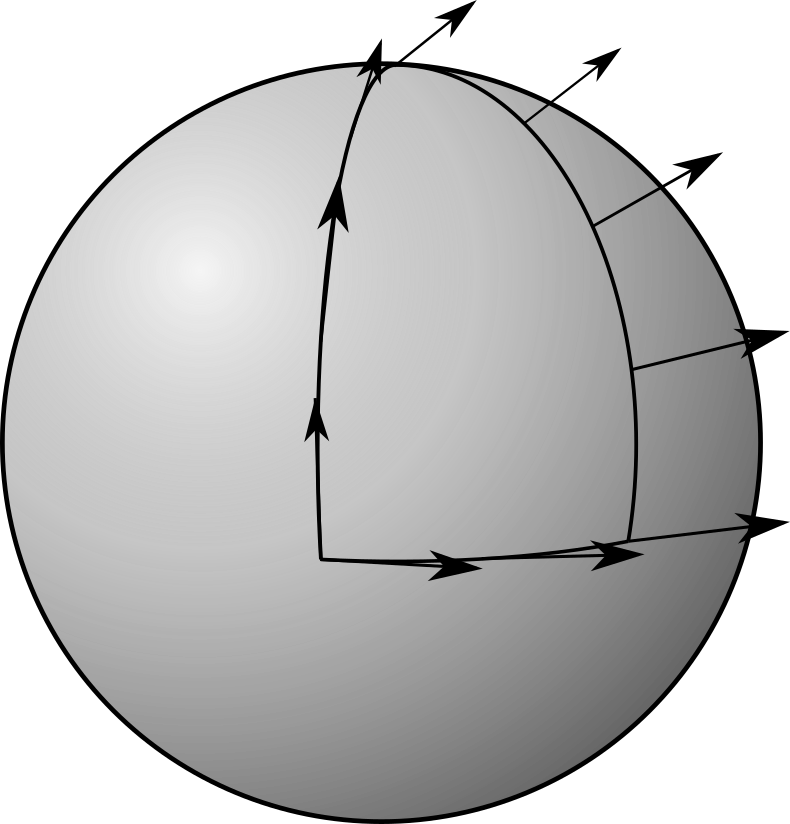
\includegraphics[scale=1]{sphereHolonomy.png}
%\end{center}

\begin{titlepage}
	\centering
	\vfill
	\vfill
	{\Large
		{\bfseries\Huge\color{ocre!80!black} Differential Geometry}\\
		\vskip1em
		Notes from Prof. I. Smith's Michaelmas 2017 Part III Course\\
		\vskip2cm
		Written by Sam Crawford\\
	}
	\vfill
	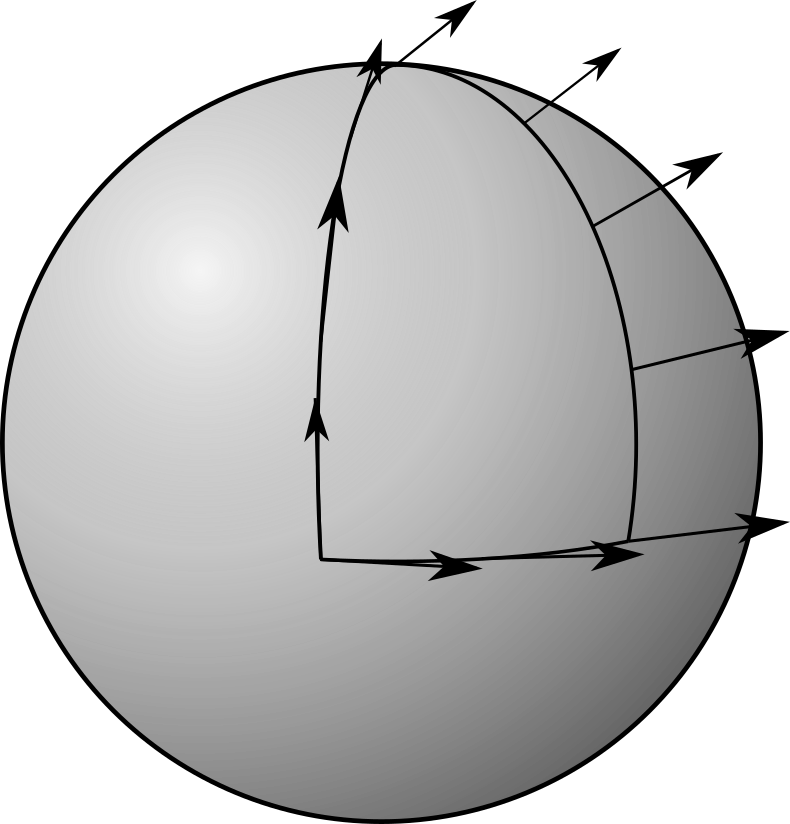
\includegraphics[width=6cm]{sphereHolonomy.png} % also works with logo.pdf
	\vfill
	\today
\end{titlepage}

\tableofcontents

\listoftodos

\chapter{Manifolds \& Vector Fields}
\section{Smooth Manifolds}

\todo[inline]{I would quite like to make this section a lot more detailed, perhaps even add in a precursory section on some of the topology required (partitions of unity etc)}

\begin{definition}[Topological Manifold]
	A \textsl{topological manifold} is a Hausdorff second countable topological space $ X $ which is locally homeomorphic to an open subset of $ \mathbb{R}^n $ for some $ n $
\end{definition}

\begin{definition}[Chart]
	A \textsl{chart} centred at $ p \in X $ is a pair $ \left( U, \phi \right) $ where $ U $ is a neighbourhood of $ p $ and $ \phi $ is a homeomorphism from $ U $ to some open subset of $ \mathbb{R}^n $.
\end{definition}

\begin{remark}
	A choice of a chart determines \textsl{local coordinates}, written $ \left\{ x_1, \ldots, x_n \right\} $, on $ X $ around $ p $.
\end{remark}

Given two charts $ (U, \phi) $ and $ (V, \psi) $ such that $ U \cap V \neq \emptyset $, we obtain a \textsl{transition function} $ \psi \circ \phi^{-1} $ from $ \phi(U \cap V) $ to $ \psi(U \cap V) $, both of which are open subsets of $ \mathbb{R}^n $.

\begin{definition}[Atlas]
	A ($ C^k $-)\textsl{atlas} on a topological manifold $ X $ is a collection of charts $ \left\{ U_\alpha, \phi_\alpha \right\}_{\alpha \in \mathcal{A}} $ such that $ \left\{ U_\alpha \right\}_\mathcal{A} $ is an open covering of $ X $ and that $ \forall \alpha, \beta \in \mathcal{A} $, ${ \phi_{\alpha\beta} \coloneqq \phi_\alpha \circ \phi_\beta^{{-1}} \in C^k }$, i.e. the transition functions are $ k $-differentiable.
\end{definition}

\begin{remark}
	By definition, topological manifolds must admit a $ C^0 $ atlas.
\end{remark}

Two atlases are \textsl{compatible} if all the transition functions between them are $ C^k $, in other words, we could combine them to obtain a new atlas. Clearly then, compatibility is a transitive property, hence it defines an equivalence class on atlases. For $ k > 0 $ such a class is referred to as a \textsl{differentiable structure}.

\begin{definition}
	A \textsl{differentiable manifold} is a topological manifold $ X $ together with a choice of a differentiable structure. If the differentiable structure contains a $ C^\infty $ atlas, then in particular we have a \textsl{smooth manifold}.
\end{definition}

\begin{definition}[Smooth Map]
	If $ M $ and $ N $ are smooth manifolds, a map $ f: M \to N $ is called \textsl{smooth} at $ p \in M $ if, for any choice of charts $ (U, \phi) $ at $ p $ and $ (V, \psi) $ at $ f(p) $, the map $ \psi \circ f \circ \phi^{-1} $ is $ C^\infty $ where defined.
\end{definition}

\begin{example}[Some Elementary Manifolds]
\hfill
	\begin{enumerate}\vspace{-1cm}
		\setcounter{enumi}{-1}
		\item $ \mathbb{R}^n $ itself is a smooth manifold, it's natural differentiable structure is the class of atlases equivalent to $ \left\{ \left( \mathbb{R}^n, \mathds{1} \right) \right\} $
		\item\label{itm:sphere} The unit sphere $ S^n $ admits a differentiable structure compatible with the pair of charts $ \left\{ \left( S^n/\{\mathbf{n}\} , \phi \right), \left( S^n/\{\mathbf{s}\} , \psi \right) \right\} $, where $ \mathbf{n} $ \& $ \mathbf{s} $ are the north and south poles of the sphere, and $ \phi $ \& represent the stereographic projections from these poles respectively.
		\item\label{itm:proj} \textsl{Real projective space}, denoted $ \mathbb{RP}^n $, is defined as an equivalence class on $ \mathbb{R}^{n+1}/\{0\} $, where $ x \sim y $ if $ \exists \lambda \in \mathbb{R}/\{0\} $ such that $ x = \lambda y $. This in fact defines a smooth manifold when equipped with the differentiable structure compatible with the atlas defined, for $ {i = 0, \ldots n} $, by
			\begin{align*}\label{key}
				U_i &= \left\{ x \in \mathbb{RP}^n : x_i \neq 0 \right\},\\
				\phi_i: U_i &\to \mathbb{R}^n, \\
				\left[x_0, \ldots, x_{n} \right] &\mapsto \tfrac{1}{x_i}\left(x_0, \ldots, x_{i-1}, x_{i+1}, \ldots, x_{n} \right).
			\end{align*}
	\end{enumerate}
\end{example}
\begin{exercise}
	Prove that the specified charts for \ref{itm:sphere} and \ref{itm:proj} are indeed smooth where they overlap.
\end{exercise}

\paragraph{}
Let $ M $ be an $ n $-manifold, and let $ N $ be a $ k $-manifold. Further, let $ f $ be a smooth map from $ M $ to $ N $. Given $ (U, \phi) $ at $ p $ and $ (V, \psi) $ at $ f(p) $, $ \psi \circ f \circ \phi^{-1}: \mathbb{R}^n \to \mathbb{R}^k $ is a smooth map between Euclidean spaces, thus it admits a Jacobian matrix: $ D( \psi f \phi^{-1} )_{\phi(p)} $. Just as in multi-variable calculus, the rank of the Jacobian (which we can show to be independent of the choices of charts) determines the nature of the map. Specifically
\begin{enumerate}
	\item The map $ f $ is an \textsl{immersion} at $ p $ if $ D $ is injective,
	\item The map $ f $ is a \textsl{submersion} at $ p $ if $ D $ is surjective,
\end{enumerate}

\begin{definition}
	Let $ i: N \hookrightarrow M $ be a smooth, injective map between manifolds. We say $ i(N) $ is a \textsl{submanifold} of $ M $ if
		\begin{enumerate}
			\item $ i $ is an immersion
			\item $ i $ is a homeomorphism from $ N $ to $ i(N) $. That is to say, it is continuous with continuous inverse with respect to the natural topology on N and the \textit{subspace topology} on $ i(N) $.
		\end{enumerate}
\end{definition}
\begin{remark}
	There are indeed some strange cases where the second condition is relevant. For example $ i: \mathbb{R} \to \mathbb{T} \simeq \mathbb{R}^2/ \mathbb{Z}^2 $ defined by $ t \mapsto [t,\alpha t] $ for some irrational number $ \alpha $ is locally injective and an immersion. But the image $ i(\mathbb{R}) $ is `dense' in $ \mathbb{T} $, and so the map is not continuous with respect to the subspace topology of $ i(\mathbb{R}) $.\todo{Clear up/make precise}
\end{remark}

\begin{definition}[Regular Value]
	Let $ f: M \to N $ be smooth. We say $ q \in N $ is a \textsl{regular value} of $ f $ if $ \forall p \in f^{-1}(q) $, we have that $ f $ is a submersion at $ p $, i.e. $ D(\psi f \phi^{-1})_{\phi(p)} $ has maximal rank.\footnote{Where unlikely to cause confusion, we will commonly adopt the shorthand where concatenation of functions represents \textit{composition} rather than multiplication.}
\end{definition}


\begin{theorem}
	Let $ f $ be a smooth map from the $ n $-manifold $ M $ to the $ k $-manifold $ N $ for $ n > k $. If $ q \in N $ is a regular value of $ f $, then $ Y \coloneqq f^{-1}(q) $ is either empty or an $ (n-k) $-dimensional submanifold of $ M $.
\end{theorem}

\todo[inline]{Implicit function theorem and slices}

\begin{proof}
%	This result is essentially an extension of the implicit function theorem from multivariable calculus, which states that if I have a function $ f $ from $ U \subset \mathbb{R}^n $ to $ V \subset \mathbb{R}^k $ such that its Jacobian is surjective at some point $ p \in U $, then there exists neighbourhoods $ \tilde{U} $ of $ p $ and $ \tilde{V} $ of $ f(p) $ and an injective function $ g: \tilde{V} \to \tilde{U} $ such that $ f \circ g = \mathrm{Id}_{\tilde{V}} $.
%
%	In our case, if we take any $ p \in f^{-1}(q) $, and charts $ (U, \phi) $ around $ p $ and $ (V, \psi) $ around $ q $, then we have a map $ \psi f \psi^{-1}: \phi(U) \to \psi(V) $ which, by hypothesis, has a surjective Jacobian. Thus, by shrinking our neighbourhoods $ U $ and $ V $ if necessary, we can define -- by the implicit function theorem -- a right inverse function $ g: \psi(V) \to \phi(U) $ such that $ \psi f \phi^{-1} g = \mathrm{Id}_{\psi(V)} $. We then assert that $ i = \phi^{-1} g \psi $ is the homeomorphic immersion needed. For this to be well defined, we must be able to show that $ i $ can be extended to all of $ f^{-1}(q) $ in a way that is independent of the charts used.
%
%	Say we have two charts $ \phi_1 $ and $ \phi_2 $, restricting relevant neighbourhoods to their intersections. If we find some injective function $ g_1 $ such that $ \psi f \phi_1^{-1} g_1 = \mathrm{Id}_{\psi(V)} $, then $ g_2 = \phi_2 \phi_1^{-1} g_1 $ will be an injective right inverse of $ \psi f \phi_2^{-1} $. From this definition we automatically have that $ \phi_1^{-1}g_1\psi = \phi_2^{-1}g_2\psi $ and thus $ i $ is well defined. Finally, we can use the open covering of $ f^{-1}(q) $ given by the atlas of $ M $ to connect any point in $ f^{-1}(q) $ to $ p $ by a sequence of overlapping open sets. Hence we can extend $ i $ defined in a neighbourhood of $ p $ to the whole of $ f^{-1}(q) $.

	This result is essentially an extension of the implicit function theorem from multivariable calculus, which states that if I have a function $ f $ from $ \mathbb{R}^n $ to $ \mathbb{R}^k $ such that its Jacobian is surjective at some point $ \mathbf{x} $, then there exists a neighbourhood $ U $ of $ \mathbf{x} $ which `factorises' into (open?) subsets $ K \in \mathbb{R}^{n-k} $ and $ W \in \mathbb{R}^k $ (i.e. $ U = K \times W $) such that, if $ \mathbf{x} = (\mathbf{r},\mathbf{s}) $ for $ \mathbf{r} \in K $ $ \mathbf{s} \in W $, then $ f(V \times \{\mathbf{s}) = \{f(\mathbf{x})\} $. In other words, $ K $ is analogous to the kernel of a surjective operator in linear algebra, and $ W $ determines which level set we are considering.

	Another result we need to consider is a way of finding submanifolds by factorising images of charts. Say we have a point $ p \in M $ contained in a chart $ (U, \phi) $ and that we can, as above, factorise $ \phi(U) = V \times W $ such that $ \phi(p) = (\mathbf{r},\mathbf{s}) $, then $ \phi^{-1}(V \times \{\mathbf{s}\}) \eqqcolon \tilde{U} $ can be used to form a chart $ \left( \tilde{U}, \pi \circ \phi|_{\tilde{U}} \right) $. Roughly speaking, we can then stitch collections of these charts together to form a submanifold of $ M $ of dimension $ \mathrm{Dim} (V) $.

	Now that the hard work has been thoroughly handwaved away, the result follows fairly straightforwardly. Let $ (U,\phi) $ be a chart around some point $ p \in f^{-1}(q) $ and $ (V, \psi) $ be a chart around $ q $ such that $ \phi(p) = 0 $ and $ \psi(q) = 0 $. By the assumption that $ q $ is regular, we know that $ \psi f \phi^{-1}: \phi(U) \to \psi(V) $ has a surjective Jacobean at $ p $. Hence we can factorise $ \phi(U) = K \times W $ such that $ \psi f \phi^{-1} \left( K \times \{0\} \right) = \{ 0 \} $. Finally, we stitch together the subsets $ \phi^{-1} \left( K \times \{0\} \right) $ of $ M $ to obtain a submanifold of dimension $ (n-k) $.

\end{proof}

\begin{remark}
	Luckily, it turns out that requiring $ q $ to be regular isn't too demanding. Sard's theorem states that if $ f: M \to N $ is smooth, then regular values of $ f $ are dense in $ N $, so `most' values are indeed regular.
\end{remark}

\section{Tangent Vectors}

\paragraph{}
Let $ \Sigma \subset \mathbb{R}^n $ be a smooth $ k $-dimensional submanifold. If $ p \in \Sigma $ and $ \gamma: (-\epsilon, \epsilon) \to \Sigma; 0 \mapsto p $ is a smooth curve. Then $ \gamma'(0) $ is a vector `tangent' to $ \Sigma $, centred on $ p $. Interestingly\todo{prove}, given two such curves $ \alpha $ and $ \beta $, we can find a third curve $ \gamma $ such that $ \gamma'(0) = \alpha'(0) + \beta'(0) $. A little more consideration can show that all such $ \gamma'(0) $ form a $ k $-dimensional affine subspace of $ \mathbb{R}^n $ centred at $ p $, which we write as $ T_p\Sigma $. Globally, we can consider the collection of all such vector spaces, written as
	\begin{equation}
		T\Sigma = \left\{ (p,v) \in \mathbb{R}^n \times \mathbb{R}^n | p \in \Sigma, v \in T_p\Sigma. \right\}
	\end{equation}

\paragraph{}
$ T\Sigma $ has the following features:
\begin{itemize}
	\item A map $ \pi: T\Sigma \to \Sigma; (p,v) \mapsto p $, known as the \textsl{canonical projection}. The preimages of $ \pi $ are called \textsl{fibres}, and are the $ k $-dimensional vector spaces $ T_p\Sigma $.
	\item We say that the projection $ T\Sigma \to \Sigma $ is \textsl{locally trivial} as, for any $ p $ in $ \Sigma $, we can find a neighbourhood $ U $ of $ p $ such that $ T\Sigma|_U \coloneqq \pi^{-1}(U) \simeq U \times \mathbb{R}^k $.
\end{itemize}

\begin{definition}[(Smooth) Vector Bundle]
	Let $ M $ be a smooth manifold, a \textsl{smooth vector bundle} $ E \overset{\pi}{\to} M $ of rank k consists of a smooth $ (n+k) $-manifold $ E $, with a submersion $ \pi: E \to M $ such that, for $ p \in M $, $ \pi^{-1}(p) \cong \mathbb{R}^k $ is a $ k $-dimensional vector space and such that $ \pi $ is locally trivial.
\end{definition}

\paragraph{Definition of tangent bundle via curves}
\begin{definition}[Germ (of a curve)]
	A \textsl{germ} of a curve on a smooth manifold $ M $ at $ p $ is an equivalence class of maps \\ $ {\gamma: (-\epsilon, \epsilon) \to  M } $, where $ \gamma \sim \tau $ if $ \exists \delta > 0 $ such that $ \gamma \equiv \tau $ when restricted to $ (-\delta, \delta) $.
\end{definition}
Then we can define the tangent bundle as an equivalence class on \textit{germs} where $ [\gamma] \sim [\tau] $ iff, given a chart at $ p $, $ (\phi \gamma)'(0) = (\phi \tau)'(0) $\todo{Show this is well defined and gives a vector space}.

\paragraph{Definition via derivations}

\begin{definition}[$ \boldsymbol{C^\infty(M)} $]
	The space of smooth functions on a manifold is an $ \infty $-dimensional vector space and is written
		\begin{equation}\label{key}
			C^\infty(M) \coloneqq \left\{ f: M \to \mathbb{R} \,|\, f \text{ is smooth } \right\}
		\end{equation}
\end{definition}

\begin{definition}[Derivation]
	A \textsl{derivation} at $ p \in M $ is a linear map $ \alpha_p: C^\infty(M) \to \mathbb{R} $ satisfying the \textsl{Leibniz rule}:
		\begin{equation}\label{key}
			\alpha_p(f \cdot g) = f(p)\alpha_p(g) + \alpha_p(g)g(p).
		\end{equation}
\end{definition}
\begin{remark}
	Note that the Leibniz rule is a linear condition, thus if two maps $ \alpha_p $ and $ \beta_p $ meet it, so too does $ (\alpha_p + \beta_p) $.
\end{remark}

\begin{lemma}[`Bump functions']\label{lem:bumpFunctions}
	Let $ p \in M $ and let $ U $ be a neighbourhood of $ p $. Then there exists a neighbourhood $ V $ of $ p $ properly contained within $ U $ ($ V \subsetneq U $) and a function $ f \in C^\infty(M) $ such that $ f|_V \equiv 1 $ and $ f|_{M/U} \equiv 0 $.
\end{lemma}
\begin{proof}[Proof (Sketch)]
	It is sufficient to check that this holds for a neighbourhood of $ 0 \in \mathbb{R}^n $. The trick is to use the fact that the piecewise function
		\begin{equation}\label{key}
			\alpha(t) \coloneqq \begin{cases}
			e^{-1/t^2} & \text{ if } t>0,\\
			0 & \text{ if } t \leq 0
			\end{cases}
		\end{equation}
	is in fact \textit{smooth} at $ t = 0 $. Thus we can add, multiply and (with caution) divide by variants of this function to obtain more smooth functions. Specifically, if we define
		\begin{equation}\label{key}
			\beta(t) \coloneqq \frac{\alpha(t)}{\alpha(t) + \alpha(1-t)}.
		\end{equation}
	Then we can finally obtain our 1D bump function
		\begin{equation}\label{key}
			\gamma(t) \coloneqq \beta(2+t) \beta(2-t).
		\end{equation}
	This function satisfies $ \gamma|{(-1,1)} \equiv 1 $, and then rapidly decays such that $ \gamma|_{\mathbb{R} / (-2,2)} \equiv 0 $. These three functions are plotted in \autoref{fig:bumpFunction}.
\end{proof}

\begin{remark}
	Liouville's theorem in complex analysis states that no function can be both holomorphic (which replaces smoothness when defining anything for complex manifolds) and bounded unless it is constant, which precludes the existence of bump functions for complex manifolds.
\end{remark}

\begin{figure}[h]
	\centering
	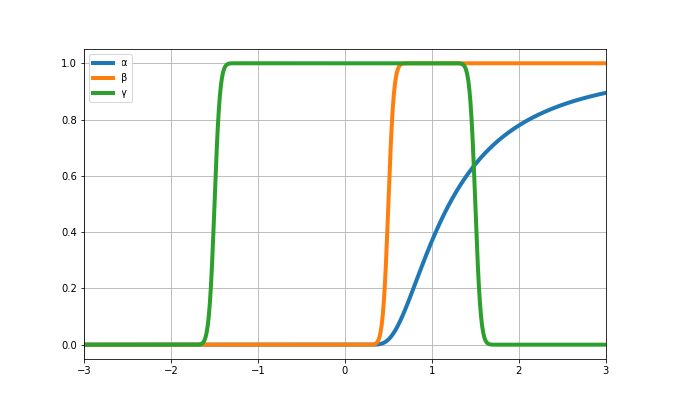
\includegraphics[width=\textwidth]{bumpFunction.png}
	\caption{The 'bump' function, along with the two functions necessary to define it. All three are smooth everywhere.}\label{fig:bumpFunction}
\end{figure}

\begin{lemma}\label{lem:derivationEquivalence}
	Let $ \ell $ be a derivation at $ p \in M $. If $ f, g \in C^\infty(M) $ and there exists a neighbourhood $ U \ni p $ such that $ f|_U \equiv g|_U $ then $ \ell(f) = \ell(g) $.
\end{lemma}

\begin{proof}
	We prove \Cref{lem:derivationEquivalence} by using a bump function. Let $ \tilde{f} \coloneqq f - g $. By \Cref{lem:bumpFunction}, we know that there exists some neighbourhood $ V $ of $ p $ and a smooth function $ h $ such that $ h(p) = 1 $ and $ h $ vanishes outside of $ V $ (more precisely, the \textit{support} of $ h $ is contained in $ V $). If we restrict our attention to the neighbourhood $ U \cap V $ of $ p $, then we know that $ \tilde{f} \equiv 0 $ and $ h \equiv 1 $. We conclude by considering the action of $ \ell $ on $ \tilde{f} \cdot h $:\todo{How do we know $ \ell(0) = \ell(\tilde{f}h) $???}
		\begin{equation}\label{key}
			\ell(\tilde{f} h ) = \ell(0) = 0.
		\end{equation}
	Thus, using the Leibniz rule:
		\begin{equation}\label{key}
			0 = \ell(\tilde{f}h) = \ell(\tilde(f))h(p) + \tilde{f}(p)\ell(h) = \ell(\tilde{f}) = \ell(f) - \ell(g),
		\end{equation}
	hence $ \ell(f) = \ell(g) $.
\end{proof}

\chapter{Differential Forms \& Connexions}
Well then, let's see how quick this is
\chapter{Geometric Structures}

\end{document}
